% Auto-generated by tools/make_fig1_tikz.py -- edit the generator, not this file.
\documentclass[border=1mm]{standalone}
\usepackage{pgfplots}
\pgfplotsset{compat=1.18}
\usepgfplotslibrary{groupplots}
\usetikzlibrary{arrows.meta,calc}

\definecolor{ink}{HTML}{1A1A1A}
\definecolor{dotgray}{HTML}{7D7D7D}
\definecolor{rowrule}{HTML}{E9E7E3}
\definecolor{refgray}{HTML}{B0ACA6}
\definecolor{reftext}{HTML}{8A8781}
\definecolor{axgray}{HTML}{444444}
\definecolor{subgray}{HTML}{6D6D6D}
\definecolor{verm}{HTML}{D55E00}
\definecolor{vermdark}{HTML}{A84A00}

\begin{document}
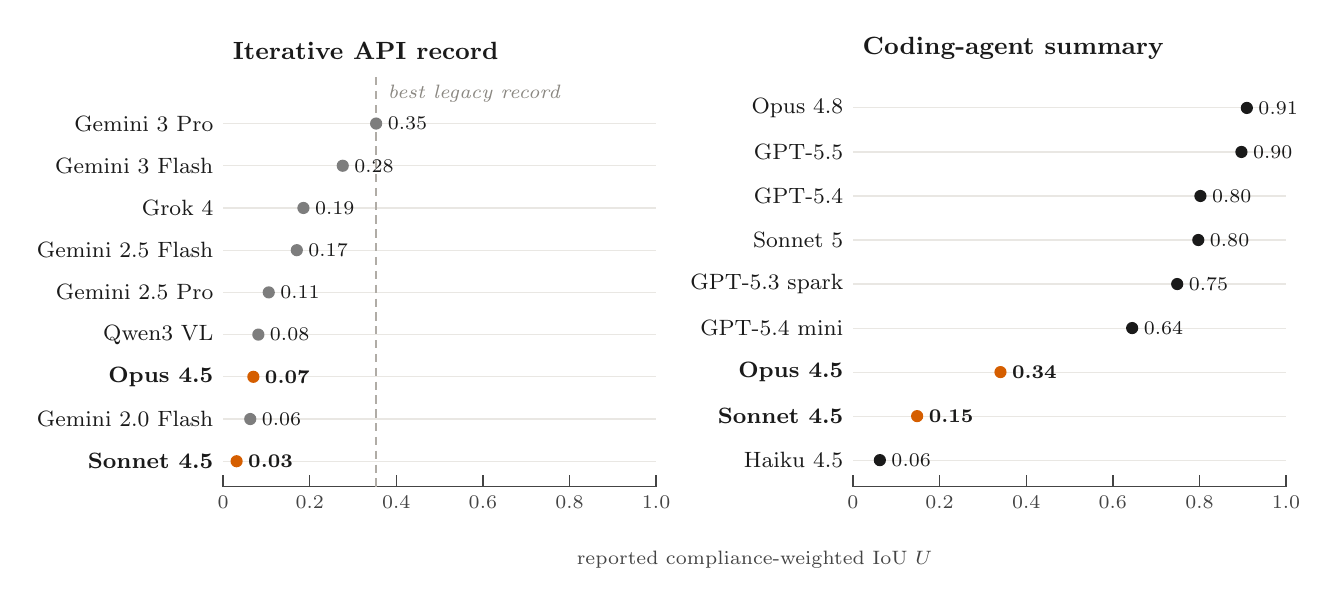
\begin{tikzpicture}
\begin{groupplot}[
  group style={group size=2 by 1, horizontal sep=25mm},
  scale only axis, width=5.5cm, height=5.2cm,
  xmin=0, xmax=1.0,
  y dir=reverse,
  ytick style={draw=none},
  yticklabel style={font=\footnotesize, text=ink},
  ymajorgrids=true,
  major grid style={line width=0.4pt, rowrule},
  axis line style={line width=0.5pt, axgray},
  axis x line*=bottom,
  xtick={0,0.2,0.4,0.6,0.8,1.0},
  xticklabels={0, 0.2, 0.4, 0.6, 0.8, 1.0},
  xticklabel style={font=\scriptsize, text=axgray},
  xtick style={line width=0.5pt, axgray},
  clip=false,
]

% ---------------- panel 1: chatbots ----------------
\nextgroupplot[
  ymin=-1.1, ymax=8.6,
  ytick={0,1,2,3,4,5,6,7,8},
  yticklabels={{Gemini 3 Pro},{Gemini 3 Flash},{Grok 4},{Gemini 2.5 Flash},{Gemini 2.5 Pro},{Qwen3 VL},{\textbf{Opus 4.5}},{Gemini 2.0 Flash},{\textbf{Sonnet 4.5}}},
  axis y line*=left,
  y axis line style={draw=none},
]
\draw[refgray, densely dashed, line width=0.6pt]
  (axis cs:0.3535,-1.1) -- (axis cs:0.3535,8.6);
\node[anchor=west, font=\scriptsize\itshape, text=reftext, inner xsep=4pt]
  at (axis cs:0.3535,-0.72) {best legacy record};
\fill[dotgray] (axis cs:0.3535,0) circle (2.2pt);
\node[anchor=west, font=\scriptsize, text=ink, inner xsep=4pt] at (axis cs:0.3535,0) {0.35};
\fill[dotgray] (axis cs:0.2764,1) circle (2.2pt);
\node[anchor=west, font=\scriptsize, text=ink, inner xsep=4pt] at (axis cs:0.2764,1) {0.28};
\fill[dotgray] (axis cs:0.1856,2) circle (2.2pt);
\node[anchor=west, font=\scriptsize, text=ink, inner xsep=4pt] at (axis cs:0.1856,2) {0.19};
\fill[dotgray] (axis cs:0.1703,3) circle (2.2pt);
\node[anchor=west, font=\scriptsize, text=ink, inner xsep=4pt] at (axis cs:0.1703,3) {0.17};
\fill[dotgray] (axis cs:0.1055,4) circle (2.2pt);
\node[anchor=west, font=\scriptsize, text=ink, inner xsep=4pt] at (axis cs:0.1055,4) {0.11};
\fill[dotgray] (axis cs:0.0815,5) circle (2.2pt);
\node[anchor=west, font=\scriptsize, text=ink, inner xsep=4pt] at (axis cs:0.0815,5) {0.08};
\fill[verm] (axis cs:0.0700,6) circle (2.2pt);
\node[anchor=west, font=\scriptsize\bfseries, text=ink, inner xsep=4pt] at (axis cs:0.0700,6) {0.07};
\fill[dotgray] (axis cs:0.0628,7) circle (2.2pt);
\node[anchor=west, font=\scriptsize, text=ink, inner xsep=4pt] at (axis cs:0.0628,7) {0.06};
\fill[verm] (axis cs:0.0313,8) circle (2.2pt);
\node[anchor=west, font=\scriptsize\bfseries, text=ink, inner xsep=4pt] at (axis cs:0.0313,8) {0.03};
\node[anchor=south west, font=\small\bfseries, text=ink, yshift=3pt]
  at (rel axis cs:0,1) {Iterative API record};

% ---------------- panel 2: agents ----------------
\nextgroupplot[
  ymin=-0.7, ymax=8.6,
  ytick={0,1,2,3,4,5,6,7,8},
  yticklabels={{Opus 4.8},{GPT-5.5},{GPT-5.4},{Sonnet 5},{GPT-5.3 spark},{GPT-5.4 mini},{\textbf{Opus 4.5}},{\textbf{Sonnet 4.5}},{Haiku 4.5}},
  axis y line*=left,
  y axis line style={draw=none},
]
\fill[ink] (axis cs:0.9095,0) circle (2.2pt);
\node[anchor=west, font=\scriptsize, text=ink, inner xsep=4pt] at (axis cs:0.9095,0) {0.91};
\fill[ink] (axis cs:0.8970,1) circle (2.2pt);
\node[anchor=west, font=\scriptsize, text=ink, inner xsep=4pt] at (axis cs:0.8970,1) {0.90};
\fill[ink] (axis cs:0.8023,2) circle (2.2pt);
\node[anchor=west, font=\scriptsize, text=ink, inner xsep=4pt] at (axis cs:0.8023,2) {0.80};
\fill[ink] (axis cs:0.7974,3) circle (2.2pt);
\node[anchor=west, font=\scriptsize, text=ink, inner xsep=4pt] at (axis cs:0.7974,3) {0.80};
\fill[ink] (axis cs:0.7487,4) circle (2.2pt);
\node[anchor=west, font=\scriptsize, text=ink, inner xsep=4pt] at (axis cs:0.7487,4) {0.75};
\fill[ink] (axis cs:0.6447,5) circle (2.2pt);
\node[anchor=west, font=\scriptsize, text=ink, inner xsep=4pt] at (axis cs:0.6447,5) {0.64};
\fill[verm] (axis cs:0.3406,6) circle (2.2pt);
\node[anchor=west, font=\scriptsize\bfseries, text=ink, inner xsep=4pt] at (axis cs:0.3406,6) {0.34};
\fill[verm] (axis cs:0.1482,7) circle (2.2pt);
\node[anchor=west, font=\scriptsize\bfseries, text=ink, inner xsep=4pt] at (axis cs:0.1482,7) {0.15};
\fill[ink] (axis cs:0.0621,8) circle (2.2pt);
\node[anchor=west, font=\scriptsize, text=ink, inner xsep=4pt] at (axis cs:0.0621,8) {0.06};
\node[anchor=south west, font=\small\bfseries, text=ink, yshift=3pt]
  at (rel axis cs:0,1) {Coding-agent summary};

\end{groupplot}
\node[anchor=north, font=\scriptsize, text=axgray, yshift=-7mm]
  at ($(group c1r1.south)!0.5!(group c2r1.south)$)
  {reported compliance-weighted IoU $U$};
\end{tikzpicture}
\end{document}
